% SVN info for this file
\svnidlong
{$HeadURL$}
{$LastChangedDate$}
{$LastChangedRevision$}
{$LastChangedBy$}

\chapter{Proprietà elettriche della materia}
\labelChapter{dielettrici}

\begin{introduction}
	‘‘BEEP BOOP''
	\begin{flushright}
		\textscsl{Lollo BiancoBOT}, dopo aver finito le citazioni. %TODO:quote 
	\end{flushright}
\end{introduction}
\lettrine[findent=1pt, nindent=0pt]{D}{opo}
\section{Materiale dielettrici e condensatori}
Consideriamo un \textit{condensatore} alle cui armature è collegato un \textit{elettroscopio}: anche lo abbiamo introdotto come strumento per misurare la carica, può essere usato (e qui lo useremo in questo secondo modo) anche per misurare la differenza di potenziale e/o il campo elettrico. Ricordiamo che il campo elettrico interno ad un condensatore piano con armature distanti $d$ e densità di carica uniforme $\sigma$ è, in modulo, pari a
\begin{equation*}
	E_0=\frac{\sigma}{\epsilon_0}
\end{equation*}
e la differenza di potenziale è
\begin{equation*}
	V_0=\frac{\sigma d}{\epsilon_0}=E_0d
\end{equation*}
Se colleghiamo (in parallelo) l'elettroscopio, tale differenza di potenziale corrisponde ad un certo angolo di separazione delle foglioline d'oro. 
\begin{center}
	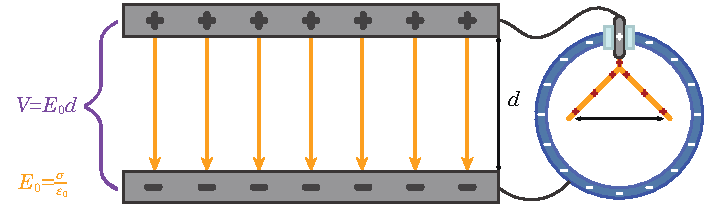
\includegraphics[width=0.75\textwidth]{images/chp6/chp6elettroscopio1.pdf}
\end{center}
\paragraph{Potenziale e capacità di un condensatore con conduttore all'interno}
Se introduciamo una \textit{lastra conduttrice} di spessore $s$ nello spazio tra le due piastre, osservando l'elettroscopio ci accorgiamo che l'angolo tra le foglioline è minore rispetto al caso precedente. Effettivamente avviene un calo di potenziale, ma perché?
\begin{center}
	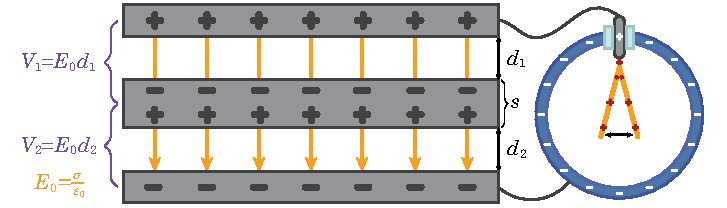
\includegraphics[width=0.75\textwidth]{images/chp6/chp6elettroscopio2.pdf}
\end{center}
Il campo elettrico del condensatore induce una separazione di carica nella lastra conduttrice, formando una distribuzione superficie di carica positiva da un lato e negativa dall'altra. Ciò induce un campo elettrico di verso opposto a quello già presente, in modo che all'interno della lastra \textit{non} ci sia campo elettrico, ma questo comporta una diminuzione del campo elettrico. In termini di potenziali, si noti che la \ddp
\begin{itemize}
	\item tra la prima piastra e il conduttore è $V_1=E_0d_1$.
	\item tra il conduttore e la seconda piastra è $V_2=E_0d_2$.
\end{itemize}
dove $d_i$ è la distanza tra la piastra $i$-esima e il conduttore; poiché $d_1+d_2=d-s$, la differenza di potenziale complessiva è
\begin{equation*}
	V_{C}=V_1+V_2=E_0\left(d-s\right)=V_0-V_{lastra}<V_0
\end{equation*}
In altre parole, la \ddp \textit{diminuisce} di un fattore $E_0s$. Se occupassi l'intera intercapedine con un materiale conduttore, è evidente che si avrebbe $V=0$: il condensatore diventerebbe un unico conduttore e le cariche si disporrebbero sulla superficie esterna.\\
Al contrario, la capacità \textit{aumenta}. Se chiamiamo la nuova capacità $C_C$, noto che $V_{C}=\dfrac{q_0}{C_C}$, si ha
\begin{equation*}
	V_C=\frac{q}{C_C}=E_0\left(d-s\right)=\frac{q}{\Sigma \epsilon_0}\left(d-s\right)\implies \frac{1}{C_C}=\frac{d-s}{\Sigma \epsilon_0}C_C=\frac{\Sigma \epsilon_0}{d-s}>\frac{\Sigma \epsilon_0}{d}=C_0
\end{equation*}
\begin{equation}
	C_C=\frac{\Sigma \epsilon_0}{d-s}>C_0
\end{equation}
\paragraph{Potenziale di un condensatore con isolante all'interno}
Ripetiamo l'esperimento con una lastra di \textit{materiale isolante}\footnote{In realtà quello che affrontiamo in questo paragrafo è vero solo alcuni tipi di isolanti, i cosiddetti \textbf{dielettrici (lineari)}; nella sezione XXX approfondiremo la differenza tra i due.}.
\begin{center}
	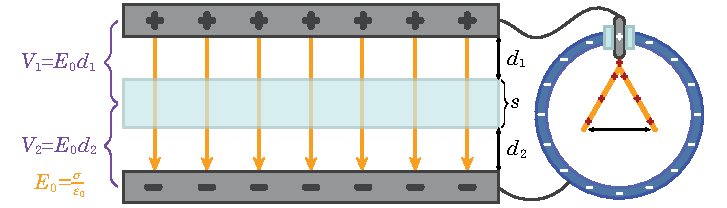
\includegraphics[width=0.75\textwidth]{images/chp6/chp6elettroscopio3.pdf}
\end{center}
Come prima, ci accorgiamo che la differenza di potenziale $V$ (e quindi il campo elettrico) è \textit{minore} del caso col vuoto nell'intercapedine; tuttavia, a parità dello spessore della lastra $s$ tale \ddp è invece \textit{maggiore} del caso con il materiale conduttore.
\begin{equation*}
	V_{C}<V<V_0
\end{equation*}
Se riempissimo tutto lo spazio intermedio con una lastra di isolante, si avrebbe $V_{\kappa}\neq0$. In particolare, si osserva che il potenziale tra le piastre in presenza di un isolante di spessore $s$ è
\begin{equation*}
	V(s)=\left(V_{\kappa}-V_0\right)\frac{s}{d}+V_0
\end{equation*} 
dove $V_{\kappa}$ indica il potenziale per $s=d$ (condensatore pieno di isolante) e $V_0$ quello per $s=0$  (condensatore vuoto).
\paragraph{Costante dielettrica relativa}
Sperimentalmente, si trova che il rapporto tra la \ddp $V_0$ misurata con il condensatore vuoto e quella $V_{\kappa}$ con il condensatore riempito di isolante è \textit{caratteristico} del \textit{tipo} di materiale, ma non dipende dalla geometria o dalla carica delle armature.
\begin{define}[Costante dielettrica relativa e suscettibilità elettrica del dielettrico]
	La \textbf{costante dielettrica relativa}\index{costante!dielettrica!relativa} è il rapporto adimensionale
	\begin{equation}
		\tcboxmath[colback=yellowpastellow!30!white,colframe=ceruleancrayola!85!black,drop fuzzy shadow, nobeforeafter, math upper, tcbox raise base, enhanced]{\kappa=\frac{V_0}{V_k}>1}
	\end{equation}
	La grandezza
	\begin{equation}
		\tcboxmath[colback=yellowpastellow!30!white,colframe=ceruleancrayola!85!black,drop fuzzy shadow, nobeforeafter, math upper, tcbox raise base, enhanced]{\chi=\kappa - 1>0}
	\end{equation}
	viene detta \textbf{suscettibilità elettrica del dielettrico}\index{suscettibilità!elettrica del dielettrico}.
\end{define}
Maggiore è $\kappa$, maggiori sono le capacità conduttive del materiale: formalmente, un materiale è un \textit{conduttore perfetto} se $\kappa=+\infty$, ossia se $V_{\kappa}=V_C=0$.

La seguente tabella presenta alcuni materiali e le loro costanti dielettriche relative.
\begin{center}
	\begin{tabular}{lc}
		\textbf{Materiale}      & \textbf{Costante dielettrica relativa} $\kappa$\\\hline
		Aria           & \num{1,00059}                                                                    \\
		Acqua          & \num{80}                                                                         \\
		Alcool etilico & \num{28}                                                                         \\
		Ambra          & \num{2,5}                                                                        \\
		Bachelite      & \num{4,9}                                                                        \\
		Carta          & \num{3,7}                                                                        \\
		Polistirolo    & \num{2,6}                                                                        \\
		Porcellana     & \num{6,5}                                                                       
	\end{tabular}
\end{center}
\paragraph{Capacità di un condensatore con isolante all'interno}
Come per il caso del conduttore, la capacità \textit{aumenta}:
\begin{equation*}
	C_{\kappa}=\frac{q}{V_{\kappa}}=\frac{q\kappa}{V_0}=\kappa C_0
\end{equation*}
\begin{equation}
	C_{\kappa}=\kappa C_0>C_0
\end{equation}
\paragraph{Campo elettrico nel condensatore con isolante all'interno}
Se il potenziale del condensatore completamente riempito di isolante è minore, anche il campo elettrico è ridotto rispetto al caso senza isolante; si vede, infatti, che
\begin{equation*}
	E_{\kappa}=\frac{V_k}{d}=\frac{V_0}{\kappa d}=\frac{E_0}{\kappa}\leq E_0
\end{equation*} 
La variazione del campo elettrico dovuta alla presenza del materiale è
\begin{equation*}
	E_0-E_{\kappa}=\frac{V_0}{d}-\frac{V_0}{\kappa d}=\frac{V_0}{d}\frac{\kappa-1}{\kappa}=E_0\frac{\kappa - 1}{\kappa}
\end{equation*}
Se la densità di carica è $E_0=\dfrac{\sigma_0}{\epsilon_0}$, si osserva che 
\begin{equation}\label{campoelettricodielettrico}
	E_{\kappa}=E_0-\frac{\kappa-1}{\kappa}E_0=\frac{\sigma_0}{\epsilon_0}-\frac{\sigma_p}{\epsilon_0}
\end{equation}
dove
\begin{equation}
	\sigma_p=\frac{\kappa-1}{\kappa}\sigma_0<\sigma_0
\end{equation}
La \eqref{campoelettricodielettrico} mostra come il campo elettrico all'interno del dielettrico si possa vedere come la \textit{sovrapposizione} di due campi elettrici nel vuoto, uno $E_0$ dovuto dalle cariche libere (distribuzione di carica $\sigma$) sulle armature, l'altro $E_p$ di intensità minore e generato da una distribuzione di carica $\sigma_p$. Le cariche che generano quest'ultimo si possono \textit{immaginare} come depositate sulle facce della \textit{lastra dielettrica}, con segno opposto a quello della carica libera sull'armatura continua - in modo per certi versi simile a quanto succede con i conduttori, ma in maniera ridotta.
\begin{center}
	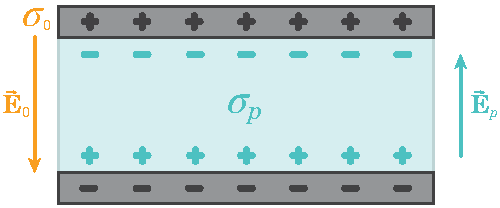
\includegraphics[width=0.6\textwidth]{images/chp6/chp6armaturedielettrico.pdf}
\end{center}
\paragraph{Costante dielettrica assoluta}
Nel \autoref{chap:leggediCoulomb} abbiamo definito la \textit{costante dielettrica del vuoto} $\epsilon_0$. Come era prevedibile dal nome, non è l'unica costante dielettrica: per trattare dei fenomeni elettromagnetici nei materiali ci conviene definire delle costanti, basate su $\epsilon_0$, che incorporano l'informazione sulla conducibilità elettrica data dalla costante dielettrica relativa $\kappa$.
\begin{define}[Costante dielettrica assoluta]
	La \textbf{costante dielettrica assoluta}\index{costante!dielettrica!assoluta} è definita come
	\begin{equation}
		\tcboxmath[colback=yellowpastellow!30!white,colframe=ceruleancrayola!85!black,drop fuzzy shadow, nobeforeafter, math upper, tcbox raise base, enhanced]{\epsilon=\kappa\epsilon_0}
	\end{equation}
\end{define}
Le formule che descrivono fenomeni elettrici nei materiali\footnote{Come già detto, questo vale solo per i dielettrici (lineari), che approfondiremo nella sezione XXX.} possono essere ottenute facilmente dal caso nel vuoto sostituendo a $\epsilon_0$ la costante assoluta $\epsilon$.
\begin{example}
	Per un condensatore piano nel vuoto si ha
	\begin{equation*}
		C_0=\frac{\epsilon_0\Sigma}{d}
	\end{equation*}
	Per un condensatore con un isolante (dielettrico) all'interno si ha
	\begin{equation*}
		C_{\kappa}=\kappa C_0=\frac{\kappa\epsilon_0\Sigma}{d}=\frac{\epsilon\Sigma}{d}
	\end{equation*}
\end{example}
\begin{observe}
	In generale, si può calcolare la costante dielettrica \textit{relativa} misurando la costante dielettrica \textit{assoluta} del materiale con un qualche \textit{esperimento opportuno} e dividendo per la costante dielettrica nel vuoto.
	\begin{equation}
		\kappa=\frac{\epsilon}{\epsilon_0}
	\end{equation}
\end{observe}
\section{Polarizzazione}
È noto che gli isolanti sono caratterizzati da una scarsa presenza di cariche libere, a differenza dei conduttori. Ciò farebbe presupporre che le cariche sulle facce che abbiamo immaginato nella sezione precedente come potenziale spiegazione del campo $E_p$ siano, per l'appunto, un frutto della \textit{fervida immaginazione} di un fisico.\\
In realtà tali cariche non sono per nulla fittizie, ma allo stesso tempo non sono come cariche \textit{libere} presenti nei conduttori: esse sono il risultato macroscopico di \textit{processi microscopici}, alla cui base stanno i fenomeni di \textit{polarizzazione}.

Negli isolanti, come appena detto, le cariche non sono particolarmente libere: quasi tutti gli elettroni sono legati agli atomi e non possono allontanarsi spontaneamente. Si può comunque, con l'azione di \textit{agenti esterni}, separare \textit{localmente} cariche positive e negative all'interno degli atomi - senza romperne quindi i legami - in modo da indurre una separazione di carica.

Il fenomeno della \textbf{polarizzazione}\index{polarizzazione} consiste proprio in questo: molto brevemente, esso consiste nel far acquisire alle particelle della materiale un momento di dipolo proporzionale all'effetto di un campo elettrico esterno, in modo da causare il comportamento osservato in precedenza nei dielettrici. Non esiste un \textit{unico} modo di polarizzare atomi o molecole; noi ci occuperemo della \textit{polarizzazione elettronica} e della \textit{polarizzazione per orientamento}.
\paragraph{Polarizzazione elettronica}
Approfondiamo ora il primo tipo. Un atomo, secondo il modello \textit{non quantistico}, consiste in un \textit{nucleo} positivo immerso in una \textit{nube} di elettroni negativi. In assenza di un campo elettrico esterno, il nucleo è neutro e la distribuzione degli elettroni attorno al nucleo è mediamente simmetrica, in modo che il centro di massa della nube coincida con la posizione del nucleo.
\begin{center}
	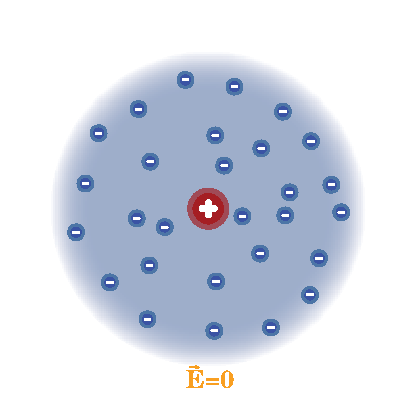
\includegraphics[width=0.35\textwidth]{images/chp6/chp6polarizzazionenucleo1.pdf}
\end{center}
Introducendo il campo elettrico, la nube negativa subisce uno spostamento \textit{contro} il campo elettrico, mentre il nucleo positivo si sposta in senso \textit{concorde} al campo fino a raggiungere una nuova posizione di equilibrio in cui il campo elettrico è \textit{controbilanciato} dall'attrazione di \textit{dipolo} tra cariche di segno opposto.
\begin{center}
	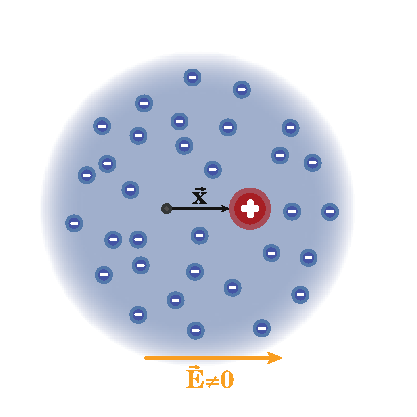
\includegraphics[width=0.35\textwidth]{images/chp6/chp6polarizzazionenucleo2.pdf}
\end{center}
All'equilibrio, tra i due centri di cariche c'è una distanza $\vba{x}$, con cui definiamo il \textbf{momento di dipolo elettrico} della configurazione ottenuta.
\begin{equation}
	\tcboxmath[colback=yellowpastellow!30!white,drop fuzzy shadow, nobeforeafter, math upper, tcbox raise base, enhanced]{\vba{p}_a=q\vba{x}=Ze\vba{x}}
\end{equation}
dove $Z$ è il numero di cariche nell'atomo e $\vba{x}$ va del centro di carica negativa a quello positiva - ossia nella direzione del campo elettrico.
\begin{observe}
	Si noti che nel singolo atomo tale spostamento è dell'ordine di $\num{10d-15}$, pari circa alle dimensioni del nucleo e quindi il momento di dipolo è \textit{davvero piccolo}. Tuttavia, poiché gli atomi per unità di volume sono un numero estremamente elevato, l'effetto complessivo in un materiale è invece \textit{misurabile}.
\end{observe}
La \textbf{polarizzazione per elettrizzazione}\index{polarizzazione!per elettrizzazione} funziona sinteticamente così: un atomo soggetto ad un campo elettrico esterno $\vba{E}$ acquista un momento di dipolo $\vba{p}_a$ elettrico microscopico, parallelo e concorde al campo $\vba{E}$.
\begin{observe}
	Per creare e mantenere questa distanza tra i centri di carica è necessaria dell'energia, fornita dal campo elettrico e che viene immagazzinata nel dipolo.
\end{observe}
\paragraph{Polarizzazione per orientamento}
Sebbene abbiamo visto come polarizzare degli atomi, ci sono alcune sostanze le cui molecole presentano già un \textit{momento di dipolo intrinseco}: questo avviene nel caso di certe molecole poliatomiche come l'\textit{acqua} $\left(\mathrm{H}_2\mathrm{O}\right)$ o l'\textit{anidride carbonica} $\left(\mathrm{CO}_2\right)$ in cui la distribuzione delle cariche - dovuta ai legami elettrostatici - è tale che il centro delle cariche negative \textit{non} coincide con quello positivo. Tali molecole, non sorprendentemente, sono dette \textbf{polari}\index{molecola!polare}.
\begin{center}
	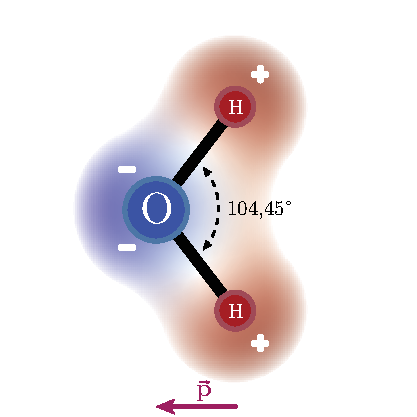
\includegraphics[width=0.4\textwidth]{images/chp6/chp6molecolaacqua.pdf}
\end{center}
\begin{minipage}{0.39\textwidth}
	\begin{center}
		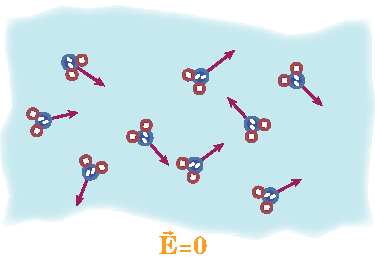
\includegraphics[width=1\textwidth]{images/chp6/chp6orientamento1.pdf}
	\end{center}
\end{minipage}\hspace{5pt}
\begin{minipage}{0.6\textwidth}
	Tuttavia, in \textit{assenza} di campo elettrico esterno i momenti di dipoli molecolari sono puramente \textit{casuali} a causa dell'agitazione termica che distrugge eventuali configurazioni ordinate con urti; il momento di dipolo medio è nullo.
	\begin{equation*}
		\left<\vba{p}\right>=0
	\end{equation*}
\end{minipage}\\
\begin{minipage}{0.39\textwidth}
	\begin{center}
		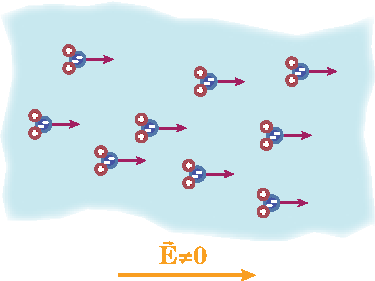
\includegraphics[width=1\textwidth]{images/chp6/chp6orientamento2.pdf}
	\end{center}
\end{minipage}\hspace{5pt}
\begin{minipage}{0.6\textwidth}
	In \textit{presenza} di un campo elettrico $\vba{E}$ esterno, i momenti di dipoli si allineano con il campo a causa del momento delle forze, facendo sì che il momento di dipolo medio risulti non nullo.
	\begin{equation*}
		\left<\vba{p}\right>\neq0
	\end{equation*}
\end{minipage}\\
Ciò nonostante, l'orientamento delle molecole è soltanto \textit{parziale} perché disturbato dall'agitazione termica: se la temperatura è bassa e il campo è intenso allora \textit{aumentano} le molecole allineate.\\
La \textbf{polarizzazione per orientamento}\index{polarizzazione!per orientamento} è quindi una polarizzazione basata sul fatto che le molecole polari sono \textit{intrinsecamente} dei dipoli.
\paragraph{Dielettrici e isolanti}\label{defdielettrico}
Prima di spiegare come queste due polarizzazioni agiscono a livello macroscopico nei materiale dielettrici, dobbiamo effettivamente spiegare cosa sia un \textit{materiale dielettrico}.

Fino ad ora abbiamo utilizzato abbastanza interscambiabilmente il termine ‘‘isolante'' e ‘‘dielettrico'', ma \textit{non} sono sinonimi.
\begin{itemize}
	\item Gli \textbf{isolanti}\index{materiale!isolante} non hanno (molti) elettroni liberi che si muovono spontaneamente. Di conseguenza, sono materiali che hanno un'alta \textit{resistività} e non scorre praticamente alcuna corrente se soggetto ad un campo esterno. Inoltre, òa costante dielettrica è minore per gli isolanti.
	\item I \textbf{dielettrici}\index{materiale!dielettrico} sono materiali isolanti le cui particelle (atomi, molecole) sono facilmente soggette a fenomeni di polarizzazione. Pertanto, immagazzinano facilmente energia nei dipoli formati.
\end{itemize}
Nei fatti, sebbene tutti i dielettrici sono isolanti, \textit{non} tutti gli isolanti sono dielettrici. Se non specificato differentemente, quando parliamo di isolanti consideriamo sempre \textit{isolanti dielettrici}.
%https://www.quora.com/What-is-difference-between-insulator-and-dielectric-substanc
\paragraph{Polarizzazione del dielettrico}
I momenti dipoli dei singoli atomi o molecole sono \textit{microscopici}. Tuttavia, l'elevato numero di particelle per unità di volume e l'alta suscettibilità alla polarizzazione fa sì che nei dielettrici questi effetti si \textit{sovrappongono} e si abbia un risultato misurabile a livello \textit{macroscopico}.

In termini espliciti, in presenza di un campo elettrico esterno $\vba{E}$ ciascun atomo o particella in un volumetto $\Delta V$ intorno ad un punto $Q$ del dielettrico acquista un momento di dipolo $\left<\vba{p}\right>$, parallelo e concorde con $\vba{E}$.
\begin{equation*}
	\left<\vba{p}\right>=\frac{1}{N}\sum_{i=1}^N\vba{p}_i
\end{equation*}
Qui $N$ è il numero di particelle nel volume $\Delta V$. La \textbf{densità di polarizzazione}\index{densità!di polarizzazione} è quindi
\begin{equation}
	\tcboxmath[colback=yellowpastellow!30!white,drop fuzzy shadow, nobeforeafter, math upper, tcbox raise base, enhanced]{\vba{P}=\frac{1}{\Delta V}\sum_{i=1}^{N}\vba{p}_i=n\left<\vba{p}\right>}
\end{equation}
dove
\begin{equation*}
	n=\lim_{\Delta V\to 0}\frac{N}{\Delta V}
\end{equation*}
è la densità di particelle nell'intorno di $Q$. Il vettore $\vba{P}$ è anche detto \textbf{vettore polarizzazione del dielettrico}\index{vettore polarizzazione!del dielettrico} e caratterizza l'effetto di formazione dei momenti di dipolo indotti dal campo esterno.

La maggior parte dei \textit{dielettrici} soddisfano una legge di proporzionalità lineare tra la densità di dipolo e il campo elettrico:
\begin{equation}
	\tcboxmath[colback=yellowpastellow!30!white,drop fuzzy shadow, nobeforeafter, math upper, tcbox raise base, enhanced]{\vba{P}=\epsilon_0\left(\kappa-1\right)\vba{E}=\epsilon_0\chi\vba{E}}
\end{equation}
I dielettrici che seguono tale legge sono detti \textbf{lineari}\index{lineari}: sono sostanze \textit{amorfe} con simmetria spaziale in tutte le direzioni (\textbf{isotropia spaziale}); in altre parole, \textit{non} ci sono direzioni preferenziali dovute \textit{a priori} dal materiale.\\
\begin{digressionwt}[Dielettrici non lineari]
	I \textit{cristalli} sono un classico esempio di dielettrici \textit{non lineari}, dato che sono \textbf{anisotropi}: $\vba{P}$ e $\vba{E}$ non sono necessariamente paralleli, ma seguono delle direzioni particolari dette \textit{assi cristallografici}. La suscettibilità elettrica, di conseguenza, non potrà essere rappresentata da un semplice numero, ma sarà rappresentata da un \textit{tensore}.
\end{digressionwt}
\begin{observe}
	Ecco spiegato il perché del termine ‘‘suscettibilità elettrica'': un materiale come l'acqua e l'alcol etilico hanno alta suscettibilità elettrica e sono proni a polarizzarsi fortemente, mentre altri come la carta o il polistirolo che hanno bassa suscettibilità tendono a polarizzarsi di meno. %TODO:check se è vero con quei materiali
\end{observe}
\begin{example}
	Ricordiamo che nel caso del condensatore si aveva
	\begin{align*}
		E_{\kappa}=\frac{E_0}{\kappa}&\text{con } E_0=\frac{\sigma}{\epsilon_0 }
	\end{align*}
	Allora, la densità di polarizzazione, in modulo, è
	\begin{equation}
		P=\epsilon_0\frac{\kappa-1}{\kappa}E_0=\sigma_0\frac{\kappa-1}{\kappa}=\sigma_p
	\end{equation}
Il vettore polarizzazione corrisponde alla densità (vettoriale) di cariche ‘‘fittizia'' definita precedentemente.
\end{example}
\subsection{Campo elettrico generato dalla polarizzazione}
Dopo aver visto come il vettore di polarizzazione sia legato ad un campo elettrico esterno, ci interessa capire come funziona il campo \textit{generato dal dielettrico polarizzato} e quale sia il legame con il vettore di polarizzazione.
\paragraph{Il caso uniforme}
Consideriamo nuovamente il caso del condensatore piano con all'interno un dielettrico \textit{polarizzato uniformemente}, ossia tale per cui $\vba{P}=\text{const}$: possiamo suddividere la lastra di dielettrico in prismi infinitesimi di base $d\Sigma$, altezza $dh$ e volume $dV=d\Sigma dh$. Ciascuno di essi contiene un certo numero di particelle orientate, per cui ad ogni prisma infinitesimo è associato un suo momento di dipolo complessivo
\begin{equation*}
	d\vba{p}=\vba{P}dV=\abs{\vba{P}}d\Sigma d\vba{h}
\end{equation*}
dove $d\vba{h}$ è concorde con la densità di polarizzazione $\vba{P}$. Ricordiamo che \textit{distribuzioni di cariche differenti} ma con \textit{stesso momento di dipolo} sono esternamente \textit{indistinguibili} l'una dall'altra; è dunque perfettamente \textit{equivalente} rimpiazzare l'effetto di moltissimi dipoli microscopici interni al prisma $dV$ con un sistema costituito da due distribuzioni di cariche
\begin{equation*}
	\pm dq_p=\pm \abs{\vba{P}}d\Sigma
\end{equation*}
poste \textit{nel vuoto}, distanti $dh$ e distribuite sulle basi del prisma con densità
\begin{equation*}
	\pm\sigma_p=\frac{\pm dq_p}{d\Sigma}=\pm\frac{\abs{\vba{P}}\Ccancel[red]{d\Sigma}}{\Ccancel[red]{d\Sigma}}=\pm\abs{\vba{P}}
\end{equation*}
dove $q_p$ è la carica ‘‘fittizia'' sulle due basi.
\begin{center}
	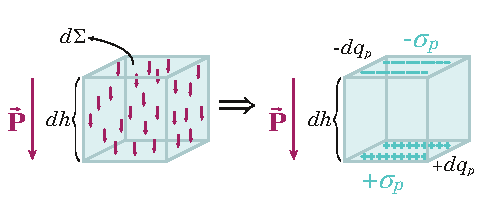
\includegraphics[width=0.6\textwidth]{images/chp6/chp6caricapolari1.pdf}
\end{center}
Siccome supponiamo $\vba{P}$ uniforme su tutto il dielettrico, il vettore di polarizzazione è lo stesso per due prismi \textit{contigui}; di conseguenza, sulle superfici di contatto le cariche sono \textit{uguali e contrarie}. Se ripetiamo questo ragionamento con altri prismi contigui alle basi, le uniche cariche rimanenti che \textit{non} sono compensate sono solo quelle sulle basi dei primi che \textit{appartengono} alla superficie del dielettrico.
\begin{center}
	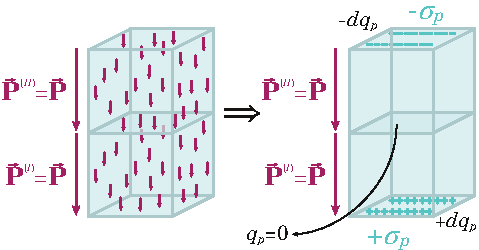
\includegraphics[width=0.6\textwidth]{images/chp6/chp6caricapolari2.pdf}
\end{center}
Quello che stiamo facendo è supporre che le cariche nel dielettrico, spostate \textit{localmente} dalle posizioni di equilibrio in quanto il materiale è \textit{polarizzato uniformemente}, si compensino all'interno ma \textit{non} all'esterno dato che la superficie di bordo non permette ulteriori compensazioni. Generalizzando ad un dielettrico di \textit{forma qualunque}, le cariche si distribuiscono sulla superficie con densità
\begin{equation}
	\tcboxmath[colback=yellowpastellow!30!white,drop fuzzy shadow, nobeforeafter, math upper, tcbox raise base, enhanced]{\sigma_p=\vba{P}\vdot \vbh{u}_n}
\end{equation}
dove $\vbh{u}_n$ è il versore normale alla superficie $\Sigma$ del materiale.
\begin{attention}
	Sebbene a tratti ciò possa ricordare il comportamento dei conduttori, il funzionamento è \textit{fondamentalmente} differente. Le \textbf{cariche di polarizzazione}\index{carica!di polarizzazione} \textit{non} sono libere come nei conduttori e quelle che notiamo sulla superficie non sono elettroni che si sono raccolti lì da altre parti del materiale, ma sono gli elettroni \textit{già presenti superficialmente}: li notiamo solo in virtù degli \textit{spostamenti locali} negli atomi e nelle molecole.\\
	Questo è il motivo per cui non possiamo \textit{asportare un pezzo} di dielettrico e misurare le cariche superficiali, come potremmo fare ad esempio con un conduttore - il funzionamento è più vicino a quello che studieremo dei \textit{magnete}, da questo punto di vista.
\end{attention}
\noindent La carica - che avevamo erroneamente definito ‘‘fittizia'' - in una particolare porzione di superficie $\Sigma_0$ è
\begin{equation}
	q=\int_{\Sigma_0}\sigma_pd\Sigma=\int_{\Sigma_0}\vba{P}\vdot \vbh{u}_nd\Sigma
	\end{equation}
\begin{observe}
	Se la polarizzazione è \textit{uniforme} non si manifestano cariche all'interno del dielettrico, quindi la carica totale sulla superficie \textit{deve} essere nulla:
	\begin{equation*}
		0=\int_{\Sigma} \sigma_p d\Sigma=\int_\Sigma \vba{P}\vdot\vbh{u}_nd\Sigma
	\end{equation*}
	Applicando il teorema della divergenza si ottiene che
	\begin{equation}
		\int_{V}\div{\vba{P}}dV=0
	\end{equation}
\end{observe}
\paragraph{Il caso \textit{non} uniforme}
Se il vettore di polarizzazione \textit{non} è uniforme, la carica di polarizzazione \textit{non} si distribuisce solo sulla superficie. Consideriamo sempre la suddivisione in prismi infinitesimi, in modo che in ogni prisma il vettore di polarizzazione ha un valore costante. Studiamo il valore della carica sulla \textit{base comune} a due prismi contigui, con asse parallelo all'asse $z$ e area di base $d\Sigma=dxdy$: a carica su una superficie infinitesima essa è
\begin{equation*}
	dq(z)=\sigma_pd\Sigma=\vba{P}\vdot \vbh{u}_nd\Sigma
\end{equation*}
La carica infinitesima sulla base è data dalla carica complessiva, sommando con segno quella presente sulla faccia inferiore $(I)$ e superiore $(II)$:
\begin{equation*}
	dq_{p}(z)=dq^{(I)}(z)-dq^{(II)}(z)=dq(z)-dq(z+dz)
\end{equation*}
Ricordiamo che il versore $\vbh{u}_n$ è preso orientato verso l'esterno della superficie; nel nostro caso,
\begin{equation*}
	\vbh{u}_n=\begin{cases}
		\vbh{u}_z&\text{per la faccia}\ (I)\\
		-\vbh{u}_z&\text{per la faccia}\ (II)\\
	\end{cases}
\end{equation*}
Se sul lato $(I)$ si ha il vettore di polarizzazione $\vba{P}^{(I)}=\vba{P}(z)$, mentre su quello $(II)$ si ha $\vba{P}^{(II)}=\vba{P}(z+dz)$, otteniamo
\begin{align*}
	-dq^{(II)}&=\vba{P}^{(II)}\vdot \vbh{u}_nd\Sigma=-P^{(II)}_z dxdy\\
	dq^{(I)}&=\vba{P}^{(I)}\vdot \vbh{u}_nd\Sigma=P^{(I)}_z dxdy\\
	dq_{p}&=dq^{(I)}-dq^{(II)}=-\left(P^{(II)}_z-P^{(I)}_z\right) dxdy
\end{align*}
\begin{center}
	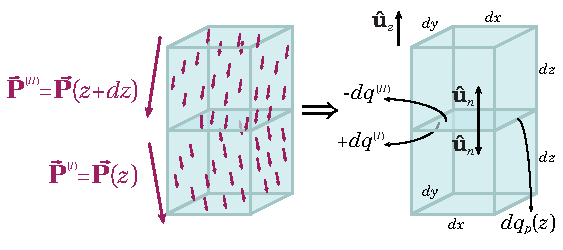
\includegraphics[width=0.75\textwidth]{images/chp6/chp6caricapolari3.pdf}
\end{center}
Poiché stiamo considerando una variazione infinitesima di $P_z$ - l'unica componente variabile di $\vba{P}$ - da un lato all'altro della superficie, questo equivale a considerar la \textit{derivata direzionale} per l'elemento infinitesimo di spessore, dato che\footnote{Ricordiamo che $dz$ è un infinitesimo e per sua definizione è una quantità tendente a zero: ai nostri fini pratici la derivata così scritta è la stessa che si incontra nei corsi di Matematica... sebbene sia ovviamente una formulazione poco rigorosa.}
\begin{equation*}
	\pdv{P_z}{z}=\frac{P(z+d z)-P(z)}{dz}=\frac{P^{(II)}_z-P^{(I)}_z}{dz}
\end{equation*}
da cui segue
\begin{equation*}
	dq_{p}(z)=-\pdv{P_z}{z}dxdydz
\end{equation*}
Se $\vba{P}$ varia lungo l'asse $z$ allora \textit{non avviene} la compensazione di cariche e le cariche di polarizzazioni appaiono anche \textit{all'interno} del dielettrico.\\
In generale, dentro ad un volumetto $dV=dxdydz$ c'è una carica di polarizzazione pari a
\begin{equation*}
	dq_{p}=\left(-\pdv{P_x}{x}-\pdv{P_y}{y}-\pdv{P_z}{z}\right)dxdydz=-\div{\vba{P}}dV
\end{equation*}
distribuita con densità volumica
\begin{equation}
	\tcboxmath[colback=yellowpastellow!30!white,drop fuzzy shadow, nobeforeafter, math upper, tcbox raise base, enhanced]{\rho_p=\frac{dq_{p}}{dV}=-\div{\vba{P}}}
\end{equation}
Anche in questo caso la carica totale di polarizzazione deve essere nulla...
\begin{equation}
	\int_V\rho_p dV+\int_{\partial V}\sigma_p d\Sigma=0
\end{equation}
... ma tale relazione ci riporta al \textit{teorema della divergenza}:
\begin{equation}
	\int_V \div{\vba{P}} dV = \int_{\partial V} \vba{P}\vdot\vbh{u}_nd\Sigma
\end{equation}
\begin{attention}
	Le distribuzioni di cariche \textit{superficiali} e \textit{spaziali} si compensano \textit{globalmente}, non localmente!
\end{attention}
\section{Le equazioni di Maxwell per l'elettrostatica nei materiali dielettrici}\label{EqMaxwellDielettrici}
Siamo ora in grado di formulare le equazioni dell'elettrostatica nei materiali dielettrici: dovremo modificare quelle leggi che presentano al loro interno informazioni riguardo le sorgenti di campo.\\
Consideriamo un campo elettrostatico $\vba{E}$. Mentre il rotore del campo elettrico rimane nullo...
\begin{equation}
	\curl{\vba{E}}=0
\end{equation}
... la sua divergenza risulta pari alla densità di carica complessiva $\rho_{tot}$ nel materiale, diviso per $\epsilon_0$ - ma tale densità è pari alla somma della densità $\rho$ già presente e della carica da polarizzazione $\rho_p$:
\begin{equation*}
	\div{\vba{E}}=\frac{\rho_{tot}}{\epsilon_0}=\frac{\rho+\rho_p}{\epsilon_0}=\frac{\rho}{\epsilon_0}-\frac{\div{\vba{P}}}{\epsilon_0}\implies \div{\left(\epsilon_0\vba{E}+\vba{P}\right)}=\rho
\end{equation*}
Definito il \textbf{campo elettrostatico di induzione dielettrica}\index{campo!elettrostatico!di induzione dielettrica}
\begin{equation}
	\tcboxmath[colback=yellowpastellow!30!white,drop fuzzy shadow, nobeforeafter, math upper, tcbox raise base, enhanced]{\vba{D}=\epsilon_0\vba{E}+\vba{P}}
\end{equation}
otteniamo la legge
\begin{equation}
	\tcboxmath[colback=yellowpastellow!30!white,drop fuzzy shadow, nobeforeafter, math upper, tcbox raise base, enhanced]{\div{\vba{D}}=\rho}\label{SecondaMaxwellDIelettriciUno}
\end{equation}
Ci sembrerebbe di aver fatto ‘‘sparire'' le cariche di polarizzazioni riscrivendo la \textit{legge di Gauss} in questa maniera, ma in realtà le abbiamo soltanto nascoste sotto il tappeto!\footnote{Con grande gioia di chi dovrà lavarlo.} I campi $\vba{E}$ e $\vba{D}$ sono legati ancora dalla densità di polarizzazione $\vba{P}$ - che incorpora in essa le informazioni della carica di polarizzazione. Per poter risolvere \textit{definitivamente} $\vba{E}$ e $\vba{D}$ ci un'\textbf{equazione di stato del mezzo dielettrico}\index{equazione!di stato!del mezzo dielettrico} che leghi esplicitamente $\vba{E}$ e $\vba{P}$ o, equivalentemente, $\vba{D}$ e $\vba{P}$.\\
Nel caso dei \textit{dielettrici lineari}, tale legge l'abbiamo già incontrata:
\begin{equation*}
	\vba{P}=\epsilon_0\left(\kappa-1\right)\vba{E}=\epsilon_0\chi\vba{E}
\end{equation*}
Da essa ricaviamo
\begin{equation}
	\tcboxmath[colback=yellowpastellow!30!white,drop fuzzy shadow, nobeforeafter, math upper, tcbox raise base, enhanced]{\vba{D}=\kappa\epsilon_0\vba{E}=\epsilon\vba{E}}
\end{equation}
e la \eqref{SecondaMaxwellDIelettriciUno} si può riscrivere come
\begin{equation}
	\tcboxmath[colback=yellowpastellow!30!white,drop fuzzy shadow, nobeforeafter, math upper, tcbox raise base, enhanced]{\div{\vba{E}}=\frac{\rho}{\epsilon}}
\end{equation} 
\begin{observe}
 Come abbiamo osservato in altri casi lavorando con i dielettrici \textit{lineari}, l'ultima legge è pari all'analoga equazione dell'elettrostatica nel vuoto a cui abbiamo sostituito a $\epsilon_0$ la costante assoluta $\epsilon$.
\end{observe}
Ricapitolando, si hanno le seguenti leggi nel caso di un dielettrico qualunque...
\begin{center}
	\begin{tabular}{p{0.22\textwidth}|c|c}
		%\multicolumn{2}{c}{\textbf{---}} \\\hline  >{\centering}
		\centering{\textbf{Nome}} &
		\textbf{Forma integrale} &
		\begin{tabular}{@{}c@{}} \textbf{Forma} \\ \textbf{differenziale}\end{tabular} \\ \hline
		
		\begin{tabular}[c]{@{}p{0.22\textwidth}@{}}	
			\\[-2mm]\textbf{Legge di Gauss per l'elettricità}\\[-2mm]~
		\end{tabular}
		&
		\begin{tabular}[c]{@{}c@{}}
			\\[-2mm]
			$\displaystyle\Phi_{\partial V}(\vba{D})=\int_{\partial V}\vba{D}\vdot\vbh{u}_nd\Sigma=q_{int}=\int_{V}\rho dV$\\[-2mm]~
		\end{tabular} &
		\begin{tabular}[c]{@{}c@{}}
			\\[-2mm]
			$\displaystyle\div{\vba{D}}=\rho$\\[-2mm]~
		\end{tabular} \\ \hline
		\begin{tabular}[c]{@{}p{0.22\textwidth}@{}}	
			\\[-2mm] \textbf{Legge dell'induzione di Faraday}\\[-2mm]~
		\end{tabular} &
		\begin{tabular}[l]{@{}l@{}}
			\\[-3mm]
			$\displaystyle\Gamma_{\gamma}(\vba{E})=\oint_{\partial \Sigma} \vba{E}\vdot d\vba{s}=0$\\[-1mm]~
		\end{tabular}
		&
		\begin{tabular}[c]{@{}c@{}}
			\\[-3mm]
			$\displaystyle\curl{\vba{E}}=0$
		\end{tabular}
	\end{tabular}~\\
\begin{equation*}
	\textit{dove}\qquad\qquad\epsilon_0\vba{E}=\vba{D}-\vba{P}
\end{equation*}
\end{center}
... e le seguenti per un dielettrico lineare con \textit{costante dielettrica assoluta} $\epsilon=\kappa\epsilon_0$.
\begin{center}
	\begin{tabular}{p{0.22\textwidth}|c|c}
		%\multicolumn{2}{c}{\textbf{---}} \\\hline  >{\centering}
		\centering{\textbf{Nome}} &
		\textbf{Forma integrale} &
		\begin{tabular}{@{}c@{}} \textbf{Forma} \\ \textbf{differenziale}\end{tabular} \\ \hline
		
		\begin{tabular}[c]{@{}p{0.22\textwidth}@{}}	
			\\[-2mm]\textbf{Legge di Gauss per l'elettricità}\\[-2mm]~
		\end{tabular}
		&
		\begin{tabular}[c]{@{}c@{}}
			\\[-2mm]
			$\displaystyle\Phi_{\partial V}(\vba{E})=\int_{\partial V}\vba{E}\vdot\vbh{u}_nd\Sigma=\frac{q_{int}}{\epsilon_0}=\int_{V}\rho dV$\\[-2mm]~
		\end{tabular} &
		\begin{tabular}[c]{@{}c@{}}
			\\[-2mm]
			$\displaystyle\div{\vba{E}}=\frac{\rho}{\epsilon}$\\[-2mm]~
		\end{tabular} \\ \hline
		\begin{tabular}[c]{@{}p{0.22\textwidth}@{}}	
			\\[-2mm] \textbf{Legge dell'induzione di Faraday}\\[-2mm]~
		\end{tabular} &
		\begin{tabular}[l]{@{}l@{}}
			\\[-3mm]
			$\displaystyle\Gamma_{\gamma}(\vba{E})=\oint_{\partial \Sigma} \vba{E}\vdot d\vba{s}=0$\\[-1mm]~
		\end{tabular}
		&
		\begin{tabular}[c]{@{}c@{}}
			\\[-3mm]
			$\displaystyle\curl{\vba{E}}=0$
		\end{tabular}
	\end{tabular}
\end{center}